% 2012 福建理 19 题图：椭圆 x^2/4+y^2/3=1，F1,F2 为焦点，
% 过 F1 的直线交椭圆于 A,B，连成三角形 ABF2。
\usetikzlibrary{arrows.meta,calc}
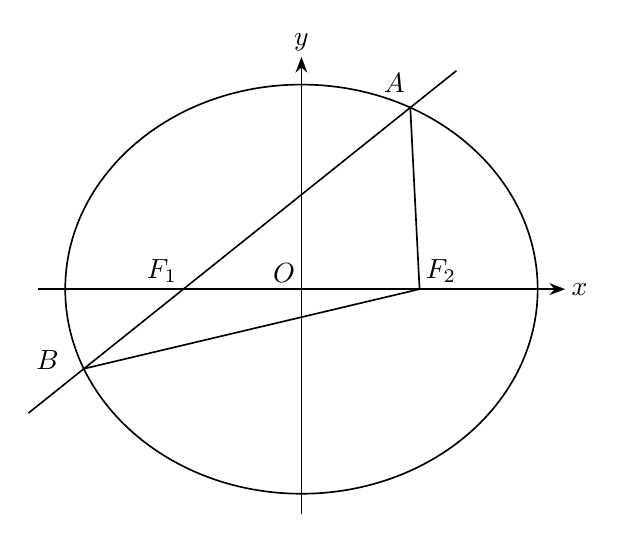
\begin{tikzpicture}[x=1cm,y=1cm,line width=.6pt,>=Stealth,font=\normalsize]
\draw[->] (-3.35,0)--(3.35,0) node[right,inner sep=2pt]{$x$};
\draw[->] (0,-2.85)--(0,2.95) node[above,inner sep=2pt]{$y$};
\draw (0,0) ellipse [x radius=3, y radius=2.5980762];
\coordinate (O)  at (0,0);
\coordinate (F1) at (-1.5,0);
\coordinate (F2) at (1.5,0);
\coordinate (A)  at (1.3823058,2.3058446);
\coordinate (B)  at (-2.7636011,-1.0108809);
\coordinate (LA) at (1.9679576,2.7743661);
\coordinate (LB) at (-3.4663827,-1.5731061);
\draw (LB)--(LA);
\draw (A)--(F2);
\draw (B)--(F2);
\node[above left,inner sep=2pt] at (O) {$O$};
\node[anchor=south east,inner sep=0pt] at (1.32,2.49) {$A$};
\node[above left,inner sep=2pt] at (F1) {$F_1$};
\node[above right,inner sep=2pt] at (F2) {$F_2$};
\node[anchor=east,inner sep=2pt] at (-3.00,-0.90) {$B$};
\end{tikzpicture}
